\section{Consultas}

A continuación, se presentan algunos ejemplos de consultas utilizadas en el proyecto, junto con sus resultados y conclusiones.
\subsection{Número total de alojamientos}
Se llevó a cabo una consulta para obtener el recuento exacto de alojamientos que se analizarán en el estudio. El propósito de esta consulta es obtener una visión general del crecimiento de los alojamientos en Málaga.  Esto es útil para comprender la competencia en el mercado y analizar la disponibilidad de alojamientos. A continuación se muestra el código utilizado y los resultados obtenidos:

\begin{verbatim}
SELECT COUNT(*) AS total_listings
FROM listings;
\end{verbatim}

La ejecución de esta consulta reveló que en la ciudad de Málaga existe un total de 7,534 alojamientos disponibles. Este dato es fundamental para comprender la dimensión y disponibilidad del mercado de alquileres vacacionales en la ciudad de Málaga.

\subsection*{Distribución geográfica de los alojamientos}

Para visualizar la distribución geográfica de los alojamientos en Málaga, se creó un mapa utilizando el software Tableau. En la figura se muestra el mapa coloreado de zonas/barrios de Málaga, con los límites de los códigos postales.

\begin{figure}[h]
    \centering
    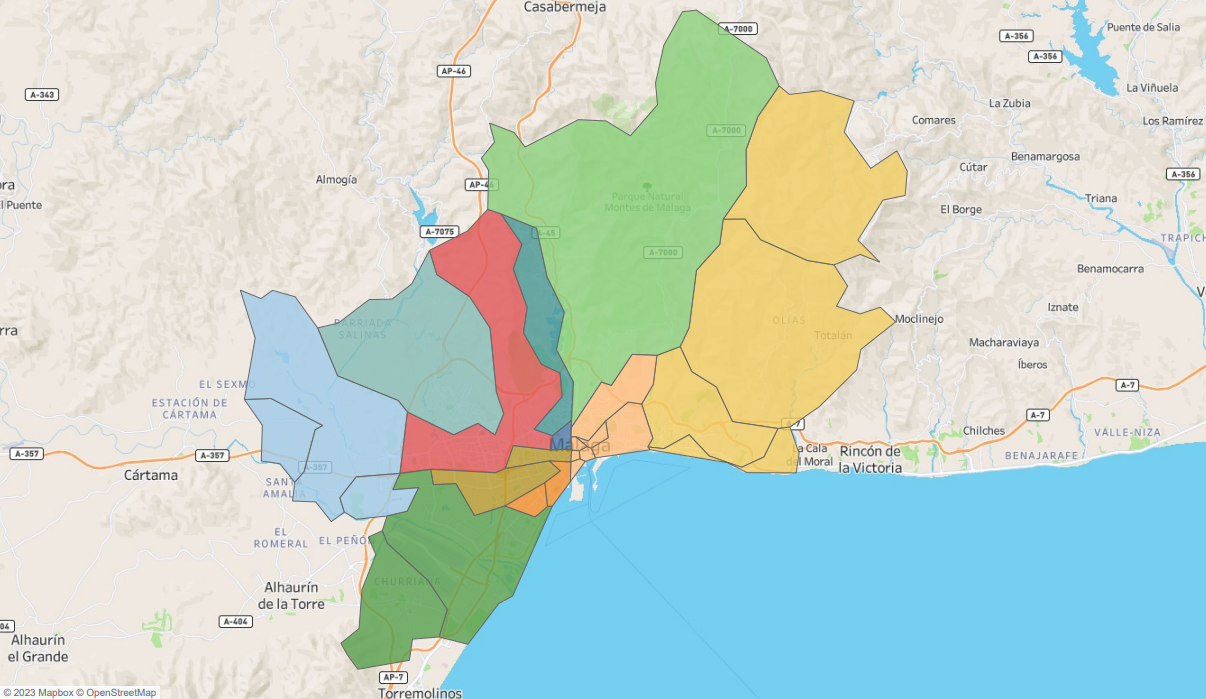
\includegraphics[width=0.9\textwidth]{capturas/1.png}
    \caption{Zonas/barrios de Málaga con límites de códigos postales.}
    \label{fig:mapa-malaga} % esto se puede usar para hacer \ref{fig:mapa-malaga} 
\end{figure}



\begin{minipage}{0.17\textwidth}
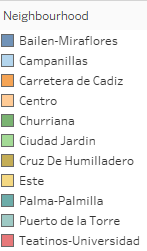
\includegraphics[width=\textwidth]{capturas/26.png}
\end{minipage}
\begin{minipage}[height=10cm,width=2cm]{11cm}
La visualización se ha segmentado en diferentes zonas o barrios de la ciudad, cada uno definido por la combinación de varios códigos postales con características similares.\\\\ 
Los límites de los códigos postales se muestran en el mapa, permitiendo una clara identificación de las áreas que abarca cada zona. Esta representación gráfica es esencial para identificar patrones de concentración y densidad de alojamientos en diferentes partes de la ciudad. La representación se basa en el modelo del proyecto \href{http://insideairbnb.com/malaga/}{Inside Airbnb}

\end{minipage}%

Los códigos postales asignados a cada zona son:
\begin{itemize}
    \item \textbf{Bailén-Miraflores}: 29009
    \item \textbf{Campanillas}: 29196, 29590, 29591
    \item \textbf{Carretera de Cádiz}: 
    \item \textbf{Centro}: 29001, 29005, 29008, 29012, 29013, 29015, 29016
    \item \textbf{Churriana}: 29004, 29140
    \item \textbf{Ciudad Jardín}: 29014
    \item \textbf{Cruz de Humilladero}: 29006, 29007
    \item \textbf{Este}: 29017, 29018, 29197, 29193
    \item \textbf{Palma-Palmilla}: 29011
    \item \textbf{Puerto de la Torre}: 29190
    \item \textbf{Teatinos-Universidad}: 29010
\end{itemize}
\ \\
En esta representación, hemos utilizado coordenadas de latitud y longitud para mapear la ubicación de los alojamientos en el espacio geográfico. Cada alojamiento se representa mediante un punto de color en el mapa, donde el color del punto se corresponde con una zona o barrio específico. Esta codificación de colores es similar a la empleada en el mapa presentado previamente.
\begin{center}
    \centering
    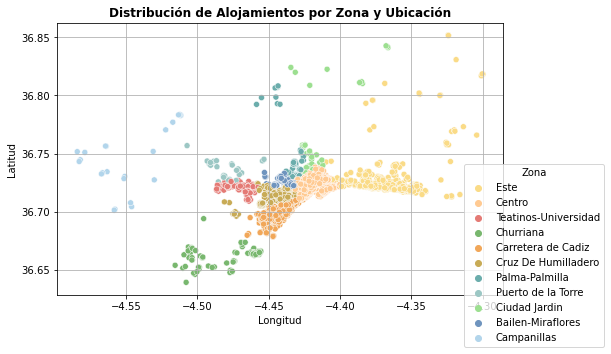
\includegraphics[width=1\textwidth]{capturas/3.png}
    \captionof{figure}{Distribución de alojamientos por zona y ubicación en coordenadas geográficas.}
\end{center}
\ \\

Esta visualización nos proporciona una visión de cómo los alojamientos se distribuyen en el entorno geográfico de Málaga. Al analizar la agrupación de puntos en diferentes zonas, podemos identificar áreas que pueden ser especialmente populares entre los huéspedes o donde los anfitriones pueden estar más activos. Asimismo, esta representación permite evaluar cómo los alojamientos se dispersan en las diversas partes de la ciudad y cómo se relaciona con los patrones observados en otras visualizaciones.\\
Observamos que existe una mayor concentración de alojamientos a medida que se aproxima al centro de la ciudad.
\newpage

Consideramos, además de la distribución geográfica de los alojamientos en Málaga, los tipos de habitaciones ofrecidos por los anfitriones. \\
\begin{center}
    \centering
    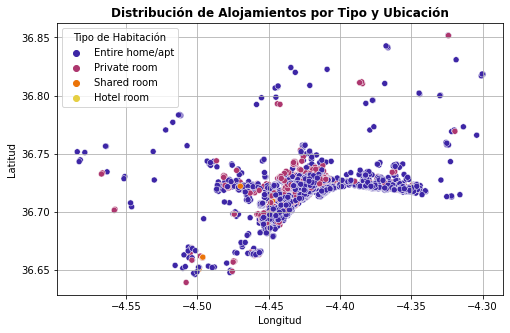
\includegraphics[width=1\textwidth]{capturas/4.png}
    \captionof{figure}{Distribución de alojamientos por tipo y ubicación en coordenadas geográficas.}
\end{center}
\ \\
Los colores de los puntos están codificados según los tipos de habitaciones, y esto nos ayuda a identificar patrones en la oferta de alojamientos, como la prevalencia de ciertos tipos de habitaciones en áreas específicas de la ciudad como las propiedades enteras o apartamentos, que son los que más abudan.\\

A continuación, se presenta una representación gráfica relacionada con la distribución de las zonas de estudio de Málaga. Observamos dos gráficas que proporcionan información sobre cómo los alojamientos se distribuyen en función del área de las zonas o barrios en Málaga y su densidad respectiva.

\begin{center}
    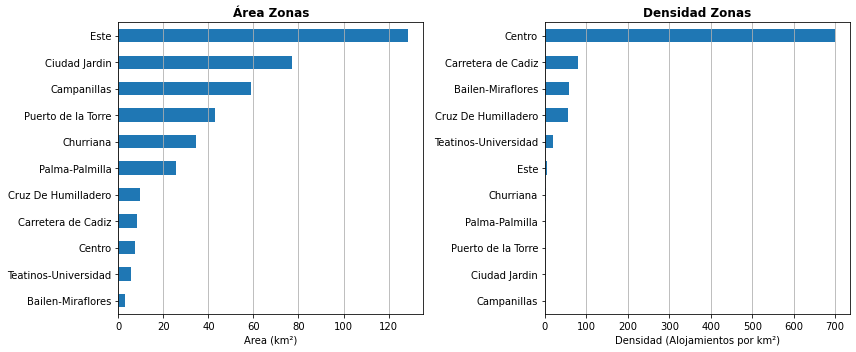
\includegraphics[width=1\textwidth]{capturas/2.png}
    \captionof{figure}{Gráficas de área y densidad de alojamientos por zona/barrio en Málaga.}
\end{center}

En la primera gráfica se muestra el \textbf{área} de cada zona o barrio en Málaga, permitiéndonos identificar visualmente cuáles son las áreas más extensas y cuáles son más compactas en términos de espacio geográfico. Esta información contextual es fundamental para comprender la distribución de los alojamientos en la ciudad y cómo podría estar relacionada con la disponibilidad de espacio.\\

La segunda gráfica representa la \textbf{densidad} de alojamientos en cada zona o barrio. La densidad se refiere al número de alojamientos por metro cuadrado en cada zona. Esta gráfica nos proporciona una perspectiva única de cómo los alojamientos se agrupan o dispersan en relación con el espacio disponible. \\\\La interacción entre ambas gráficas nos permite obtener conclusiones más precisas sobre cómo se distribuyen los alojamientos en Málaga y si hay alguna tendencia en la relación entre el área y la densidad de alojamientos.\\
Observamos que el distrito \textit{Este} es el más extenso pero no es que tiene una mayor densidad de alojamientos. Es el distrito \textit{Centro} el que tiene una mayor concentración de alojamientos por kilómetro cuadrado.

\subsection{Consulta de número de alojamientos por tipo, porcentaje del mismo , precio promedio y duración promedio de la estancia de los alojamientos por tipo}

En esta consulta, se obtuvieron datos sobre el número de alojamientos, el precio promedio y la duración promedio de la estancia según el tipo de propiedad. A continuación se muestra el código utilizado y los resultados obtenidos:
\begin{verbatim}
SELECT property_type,  COUNT(*) AS count, 
    ROUND(AVG(CAST(REGEXP_REPLACE(listings.price,
        '[^\d.]', '', 'g') AS NUMERIC))) AS avg_price, 
    ROUND(COUNT(*) * 100.0 / (SELECT COUNT(*) FROM listings), 2) 
        AS percentage, 
    ROUND(AVG(minimum_nights)) AS avg_minimum_nights
FROM listings
GROUP BY property_type 
ORDER BY count DESC;
\end{verbatim}
\begin{table}[h]
\centering
\resizebox{\textwidth}{!}{
\begin{tabular}{|l|r|r|r|r|}
\hline \textbf{Tipo} & \textbf{Nº de aloj.} & \textbf{Precio prom.} & \textbf{Porcentaje (\%)} & \textbf{Dur. prom.} \\ \hline
Entire rental unit & 5151 & 219 \texteuro & 68.37 & 3 \\ \hline
Private room in rental unit & 642 & 75 \texteuro & 8.52 & 5 \\ \hline
Entire condo & 328 & 167 \texteuro & 4.35 & 6 \\ \hline
Entire loft & 264 & 121 \texteuro & 3.50 & 5 \\ \hline
Entire home & 207 & 232 \texteuro & 2.75 & 9 \\ \hline
Entire serviced apartment & 193 & 175 \texteuro & 2.56 & 2 \\ \hline
Entire vacation home & 126 & 190 \texteuro & 1.67 & 2 \\ \hline
Private room in home & 107 & 55 \texteuro & 1.42 & 3 \\ \hline
Entire townhouse & 51 & 1741 \texteuro & 0.68 & 4 \\ \hline
... & ...& ...&...&... \\ \hline
\end{tabular}
}
\caption{Datos de alojamientos por tipo}
\end{table}
\newpage
A través de un enfoque visual, es posible resumir de manera efectiva los resultados obtenidos con respecto al precio medio según el tipo de propiedad en Málaga. Esta gráfica, generada utilizando la herramienta \textbf{Python} de \textbf{`bokeh`}, ofrece una instantánea que destaca la variabilidad en los precios de los distintos tipos de alojamientos.

\begin{center}
    \centering
    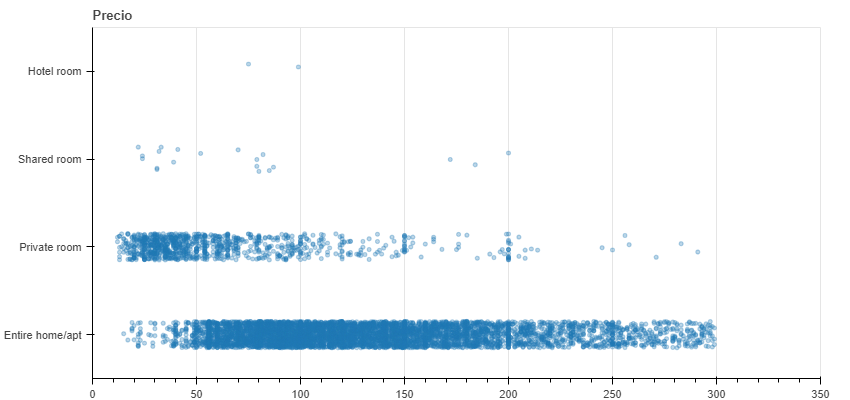
\includegraphics[width=1\textwidth]{capturas/5.png}
    \captionof{figure}{Distribución de alojamientos por precio y tipo.}
\end{center}
\begin{center}
    \centering
    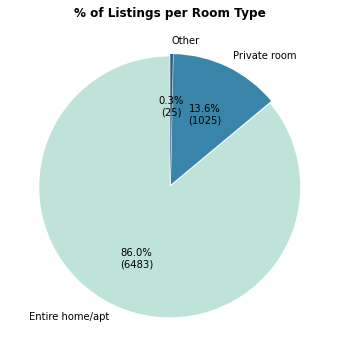
\includegraphics[width=0.5\textwidth]{capturas/14.png}
    \captionof{figure}{Porcentaje de alojamientos por tipo de habitación.}
\end{center}
El resultado revela una amplia variedad de opciones disponibles para los huéspedes. Los alquileres completos son los más comunes, seguidos de habitaciones privadas en unidades de alquiler. Los precios promedio varían según el tipo de propiedad, siendo las casas completas las más costosas. La duración promedio de la estancia también varía, con una media de 3 a 5 noches.

\subsection{Consulta de número de alojamientos por zona, porcentaje, precio promedio de los alojamientos por zona y duración promedio de la estancia de los alojamientos por zona}

En esta consulta, se obtuvieron datos relevantes sobre el número de alojamientos, el porcentaje, el precio promedio y la duración promedio de la estancia de los alojamientos por zona en Málaga. El propósito de esta consulta es analizar las características y tendencias de cada zona en relación con los alojamientos disponibles. A continuación se muestra el código utilizado y los resultados obtenidos:

\begin{verbatim}
SELECT neighbourhood_cleansed, COUNT(*) AS count, 
    ROUND(AVG(CAST(REGEXP_REPLACE(price, '[^\d.]', '', 'g') 
        AS NUMERIC))) AS avg_price,
    ROUND(COUNT(*) * 100.0 / (SELECT COUNT(*) FROM listings), 2) 
        AS percentage,
ROUND(AVG(minimum_nights)) AS avg_minimum_nights
FROM listings
GROUP BY neighbourhood_cleansed
ORDER BY avg_price DESC;
\end{verbatim}
\begin{table}[h]
\centering
\resizebox{\textwidth}{!}{
\begin{tabular}{|l|r|r|r|r|}
\hline
\textbf{Zona} & \textbf{Nº de aloj.} & \textbf{Precio prom.} & \textbf{Porcentaje (\%)} & \textbf{Dur. prom.} \\ \hline
Bailen-Miraflores & 178 & 503 \texteuro & 2.36 & 5 \\ \hline
Este & 738 & 298 \texteuro & 9.80 & 4 \\ \hline
Cruz De Humilladero & 531 & 253 \texteuro & 7.05 & 3 \\ \hline
Carretera de Cadiz & 658 & 237 \texteuro & 8.73 & 4 \\ \hline
Churriana & 101 & 182 \texteuro & 1.34 & 4 \\ \hline
Centro & 5054 & 174 \texteuro & 67.08 & 3 \\ \hline
Campanillas & 26 & 168 \texteuro & 0.35 & 3 \\ \hline
Puerto de la Torre & 31 & 156 \texteuro & 0.41 & 3 \\ \hline
Teatinos-Universidad & 105 & 127 \texteuro & 1.39 & 6 \\ \hline
Ciudad Jardin & 54 & 106 \texteuro & 0.72 & 2 \\ \hline
Palma-Palmilla & 58 & 92 \texteuro & 0.77 & 3 \\ \hline
\end{tabular}
}
\caption{Datos de alojamientos por zona}
\end{table}

Explorando más a fondo la distribución de alojamientos en Málaga, podemos utilizar una serie de gráficas para destacar aspectos clave.
Podemos analizar mediante un gráfico circular la distribución de los alojamientos en \textbf{Málaga}. 
\begin{center}
    \centering
    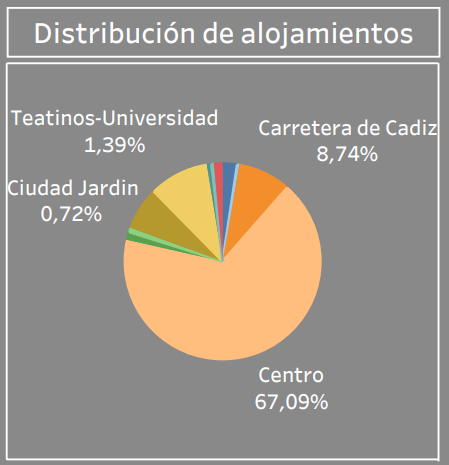
\includegraphics[width=0.4\textwidth]{capturas/6.png}
    \captionof{figure}{Distribución de alojamientos.}
\end{center}
Comprobamos que efectivamente existe una concentración mayor de alojamientos en el distrito \textit{Centro} con un $67\%$ y en segundo lugar en \textit{Carretera de Cádiz} con aproximadamente un $9\%$.\\\\
Continuamos analizando el número de alojamientos por tipo y por zona, utilizando un gráfico de barras. Es evidente que tanto las casas/apartamentos como las habitaciones privadas son las opciones más comunes en el distrito \textit{Centro}, reforzando su popularidad entre los huéspedes.
\begin{center}
    \centering
    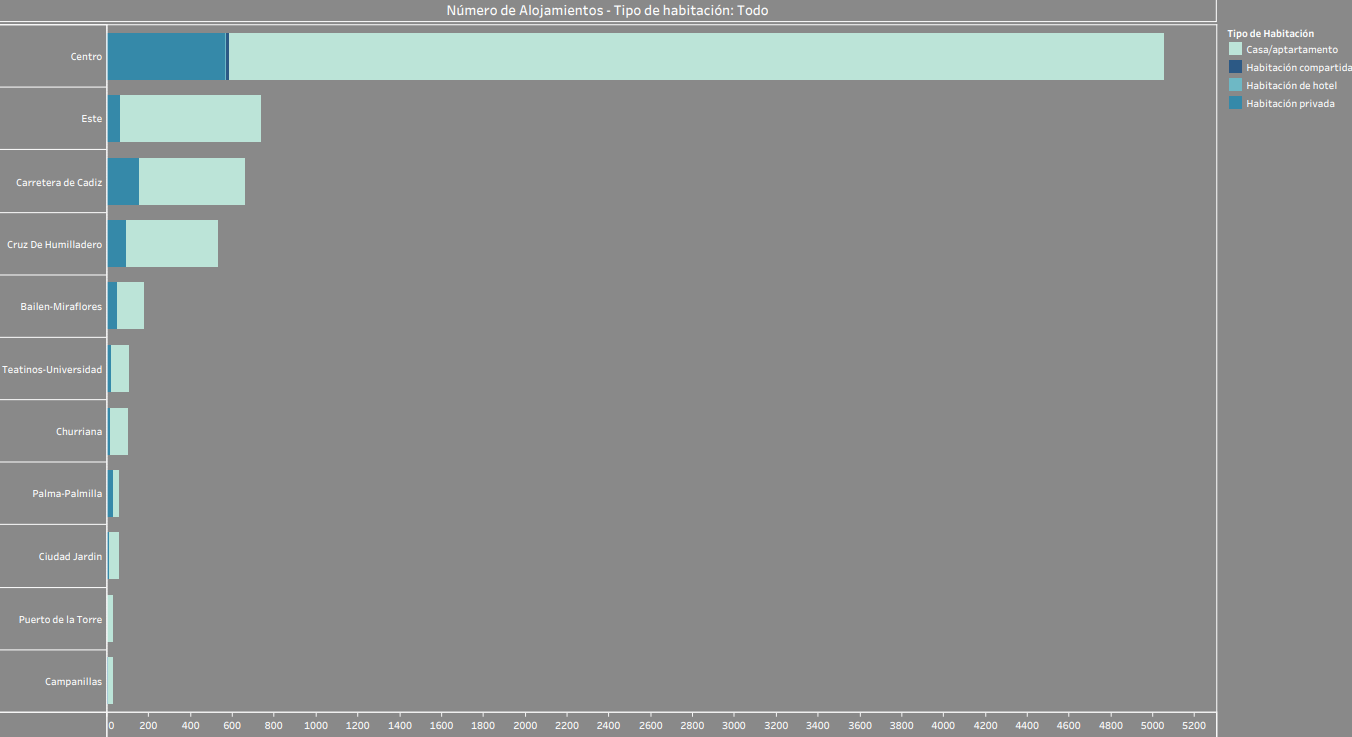
\includegraphics[width=1\textwidth]{capturas/7.png}
    \captionof{figure}{Número de alojamientos por tipo de habitación.}
\end{center}
En la siguiente gráfica se muestra la proporción de tipo de habitación en cada zona. Es esencial para conocer qué tipo de alojamiento se oferta en cada zona y permite identificar patrones.
\begin{center}
    \centering
    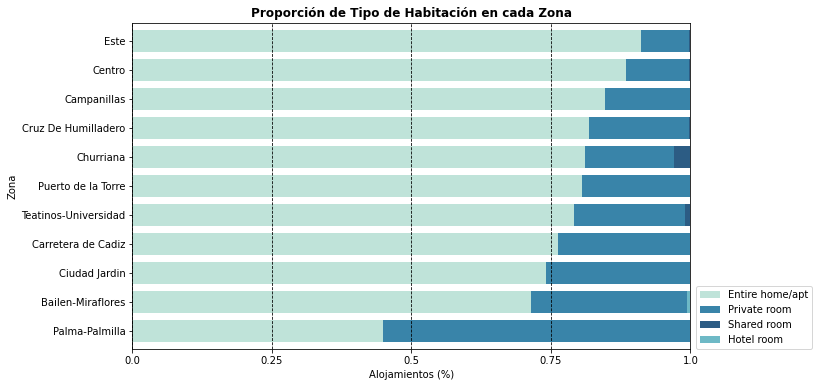
\includegraphics[width=1\textwidth]{capturas/8.png}
    \captionof{figure}{Proporción de Tipo de Habitación en cada Zona.}
\end{center}
Observamos un dato curioso: el distrito de \textit{Churriana} es el que mayor proporción de habitaciones compartidas tiene. Sin embargo, como hemos analizado anteriormente, este distrito no tiene una alta concentración de alojamientos públicos en Airbnb.
\newpage
La relación entre el precio promedio y la ubicación geográfica es crucial. Esta gráfica arroja perspectivas significativos: las zonas \textit{Bailen-Miraflores} y \textit{Este} presentan los precios más altos, mientras que \textit{Ciudad Jardin} y \textit{Palma-Palmilla} tienen precios más bajos.
\begin{center}
    \centering
    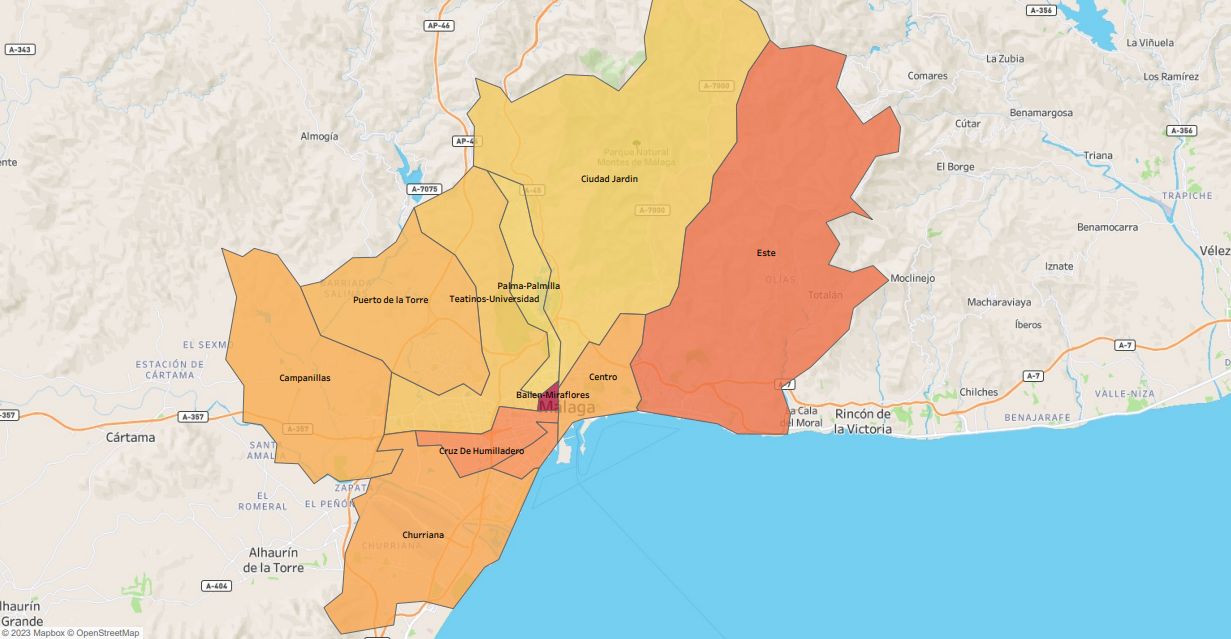
\includegraphics[width=0.95\textwidth]{capturas/9.png}
    \captionof{figure}{Precio promedio por zona.}
\end{center}
Podemos llevar a cabo un análisis más detallado desglosando los datos no solo por barrio, sino también por código postal. Este enfoque nos permitirá descubrir qué zonas específicas de Málaga presentan una mayor demanda en términos de precio.
\begin{center}
    \centering
    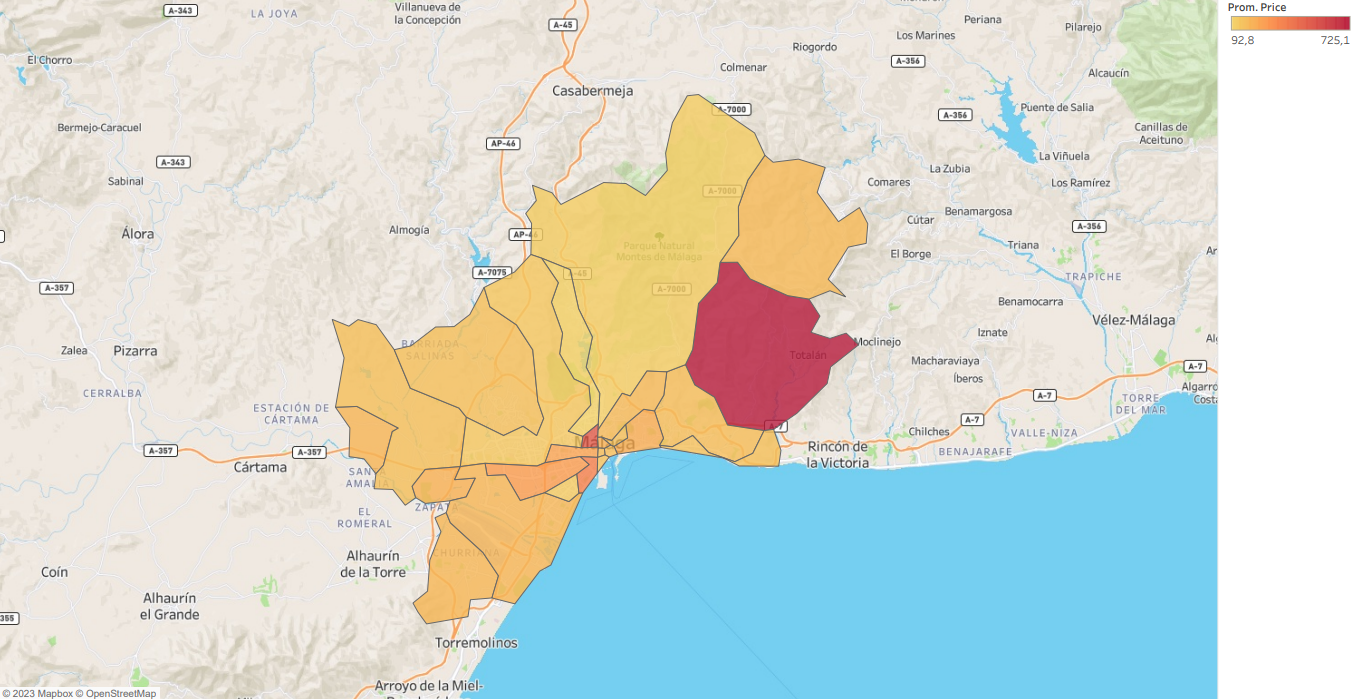
\includegraphics[width=0.95\textwidth]{capturas/10.png}
    \captionof{figure}{Precio promedio por código postal.}
\end{center}
Destacan dos códigos postales en particular: el 29197, ubicado en el distrito \textit{Este}, con un precio medio de 725,1€. Este valor sugiere una fuerte demanda en esta área específica. Otro código postal significativo es el 29009, correspondiente a \textit{Bailen Miraflores}, con un precio medio de 503,4€.\\
Finalmente, evaluamos la duración promedio de la estancia por zona. Se observa una variación entre 2 y 6 noches, resaltando la diversidad de preferencias de los huéspedes en diferentes áreas.\\
Estos resultados proporcionan una visión de la distribución geográfica de los alojamientos, los precios promedio y la duración promedio de la estancia en Málaga, siendo información relevante para entender las preferencias de los huéspedes.

\subsection{Consulta de promedio de las calificaciones}
En esta consulta, se obtiene la calificación promedio de todos los alojamientos en la ciudad de Málaga. El objetivo es determinar el nivel promedio de satisfacción de los huéspedes. A continuación se muestra el código utilizado y el resultado obtenido:
\begin{verbatim}
SELECT calculate_average_rating() AS average_rating;
\end{verbatim}

El resultado revela que la puntuación media es de 4.61. Esto indica que, en promedio, los alojamientos en Málaga han recibido una calificación alta por parte de los huéspedes.

\subsection{Consulta de los alojamientos que tienen más comentarios y su valoración}
En esta consulta, se identifican los alojamientos que han recibido la mayor cantidad de comentarios, junto con su valoración correspondiente. El objetivo es conocer los alojamientos más populares y bien valorados por los huéspedes. A continuación se muestra el código utilizado y los resultados obtenidos:
\begin{verbatim}
SELECT li.listing_url, li.name, 
    li.review_scores_rating, COUNT(*) AS comment_count
FROM reviews
JOIN listings li ON li.id = reviews.listing_id
GROUP BY li.listing_url, li.name, li.review_scores_rating
ORDER BY comment_count DESC;
\end{verbatim}
\begin{table}[h]
\centering
\resizebox{\textwidth}{!}{
\begin{tabular}{|l|l|r|r|}
\hline \textbf{Enlace del alojamiento} & \textbf{Nombre} & \textbf{Valoración} & \textbf{Nº de comentarios} \\ \hline
\href{https://www.airbnb.com/rooms/10802138}{https://www.airbnb.com/rooms/10802138} & "Room next to Airport A/C" & 4.66 & 775 \\ \hline
\href{https://www.airbnb.com/rooms/2343063}{https://www.airbnb.com/rooms/2343063} & "Nice Flat in the center VFT/MA/00202" & 4.78 & 758 \\ \hline
\href{https://www.airbnb.com/rooms/30141259}{https://www.airbnb.com/rooms/30141259} & "Apartamento Centro Málaga+Garaje Privado Gratis" & 4.76 & 672 \\ \hline
\href{https://www.airbnb.com/rooms/2336145}{https://www.airbnb.com/rooms/2336145} & "Lovely apartment in the center VFT/MA/00204" & 4.77 & 671 \\ \hline
\href{https://www.airbnb.com/rooms/18369830}{https://www.airbnb.com/rooms/18369830} & "Picasso Home" & 4.85 & 526 \\ \hline
\href{https://www.airbnb.com/rooms/6955285}{https://www.airbnb.com/rooms/6955285} & "1 Acogedora hab. cerca de la playa" & 4.54 & 521 \\ \hline
\href{https://www.airbnb.com/rooms/13315721}{https://www.airbnb.com/rooms/13315721} & "Relax, culture and beach in the heart of the city." & 4.95 & 510 \\ \hline
\href{https://www.airbnb.com/rooms/21466209}{https://www.airbnb.com/rooms/21466209} & "City Home" & 4.83 & 508 \\ \hline
... & ... & ... & ... \\ \hline
\end{tabular}
}
\caption{Alojamientos con más comentarios y su valoración}
\end{table}
Estos resultados destacan los alojamientos más populares y bien valorados en Málaga. Estos alojamientos han logrado atraer a una gran cantidad de huéspedes satisfechos y reciben una alta valoración por su calidad y servicio ofrecidos.

\subsection{Consulta del numero mínimo de noches}
En esta consulta, se busca determinar el número mínimo de noches aceptado por los alojamientos en Málaga. El objetivo es comprender la duración mínima de estadía requerida por los anfitriones. A continuación se muestra el código utilizado y el resultado obtenido:
\begin{verbatim}
SELECT calculate_max_minimum_nights() AS max_minimum_nights;
\end{verbatim}

El resultado revela que el número mínimo de noches aceptado por los alojamientos de Málaga es de 3 noches. Este dato es importante ya que indica la cantidad mínima de noches que los huéspedes deben reservar al planificar su estadía en la ciudad. Este resultado resalta la política común entre los anfitriones de exigir un mínimo de 3 noches de estancia. Con esta información, los huéspedes pueden planificar su viaje considerando esta restricción y ajustar su itinerario en consecuencia.
\newpage
\subsection{Consulta de anfitriones más activos y su relación con las revisiones}

En esta consulta, se muestra la información de los anfitriones más activos en función del número de revisiones recibidas. El objetivo es identificar a los anfitriones con mayor participación y su impacto en las revisiones de los huéspedes. A continuación se muestra el código utilizado y el resultado obtenido:

\begin{verbatim}
SELECT host_name, host_url, host_listings_count, number_of_reviews
FROM (
    SELECT DISTINCT ON (host_name, host_url)
           host_name, host_url, host_listings_count,
           number_of_reviews
    FROM listings
    ORDER BY host_name, host_url, number_of_reviews DESC
) AS subquery
ORDER BY number_of_reviews DESC;
\end{verbatim}
\begin{table}[h]
\centering
\resizebox{\textwidth}{!}{
\begin{tabular}{|l|l|r|r|}
\hline \textbf{Nombre} & \textbf{Enlace de usuario} & \textbf{Nº aloj.} & \textbf{Nº revisiones}\\ \hline
'Christina' & \href{https://www.airbnb.com/users/show/47971136}{https://www.airbnb.com/users/show/47971136} & 16 & 775 \\ \hline
'Frédéric Et Catherine' & \href{https://www.airbnb.com/users/show/11931754}{https://www.airbnb.com/users/show/11931754} & 2 & 758 \\ \hline
'Rafa\&Pilu' & \href{https://www.airbnb.com/users/show/226466430}{https://www.airbnb.com/users/show/226466430} & 3 & 672 \\ \hline
'Mónica Y Juan' & \href{https://www.airbnb.com/users/show/127195773}{https://www.airbnb.com/users/show/127195773} & 3 & 526 \\ \hline
'Sandra' & \href{https://www.airbnb.com/users/show/36462988}{https://www.airbnb.com/users/show/36462988} & 2 & 521 \\ \hline
'Carmen Y Muni' & \href{https://www.airbnb.com/users/show/15535210}{https://www.airbnb.com/users/show/15535210} & 2 & 510 \\ \hline
'Ramon' & \href{https://www.airbnb.com/users/show/32285652}{https://www.airbnb.com/users/show/32285652} & 1 & 495 \\ \hline
'Francisco' & \href{https://www.airbnb.com/users/show/44170578}{https://www.airbnb.com/users/show/44170578} & 5 & 493 \\ \hline
'Encarni' & \href{https://www.airbnb.com/users/show/47246887}{https://www.airbnb.com/users/show/47246887} & 1 & 491 \\ \hline
'Christan' & \href{https://www.airbnb.com/users/show/122669535}{https://www.airbnb.com/users/show/122669535} & 8 & 479 \\ \hline
'Lola' & \href{https://www.airbnb.com/users/show/268097476}{https://www.airbnb.com/users/show/268097476} & 3 & 472 \\ \hline
'Daniel' & \href{https://www.airbnb.com/users/show/39846040}{https://www.airbnb.com/users/show/39846040} & 2 & 459 \\ \hline
'Nataliya' & \href{https://www.airbnb.com/users/show/72851313}{https://www.airbnb.com/users/show/72851313} & 1 & 456 \\ \hline
'Rachel \& Hendrix' & \href{https://www.airbnb.com/users/show/42226210}{https://www.airbnb.com/users/show/42226210} & 1 & 455 \\ \hline
\end{tabular}
}
\caption{Anfitriones más activos y su relación con las revisiones en el año 2023}
\end{table}

\begin{center}
    \centering
    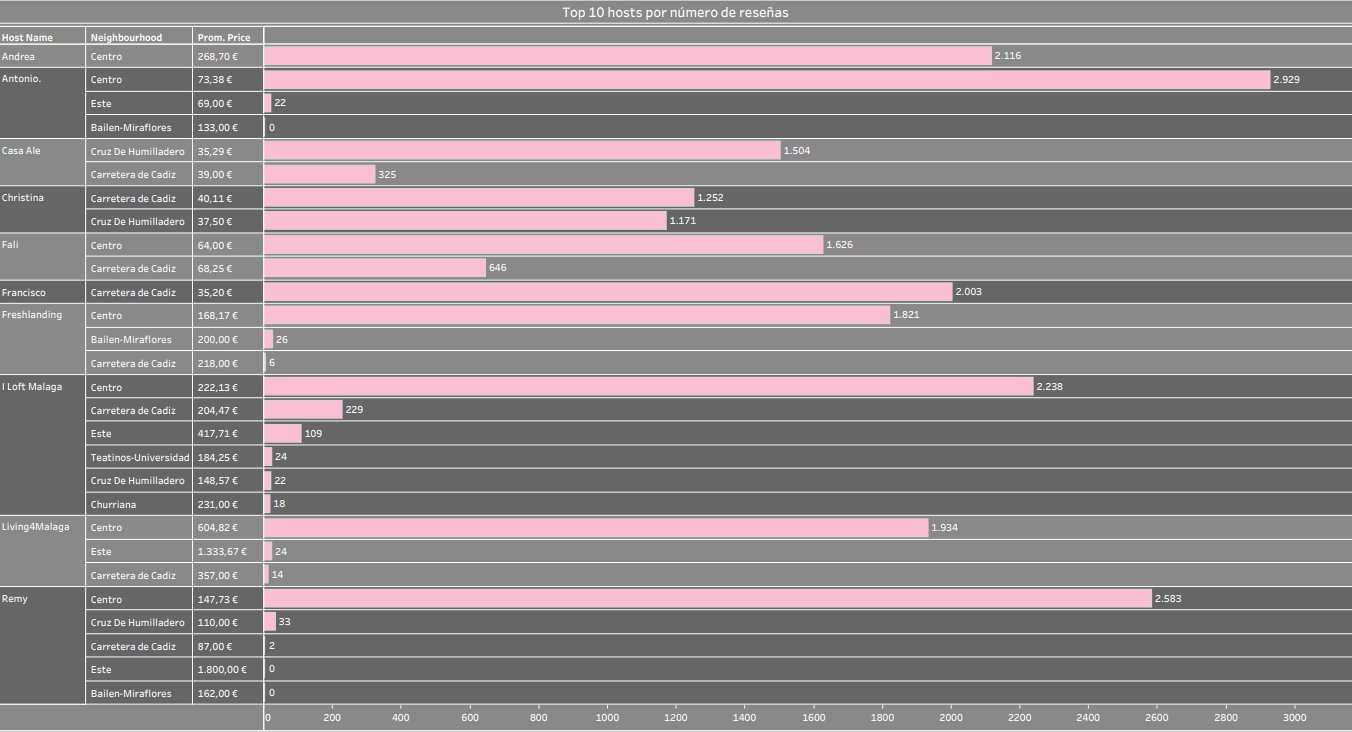
\includegraphics[width=1\textwidth]{capturas/11.png}
    \captionof{figure}{Hosts con más valoraciones junto con sus propiedades.}
\end{center}
Estos resultados destacan a los anfitriones más activos y su influencia en las reseñas de los huéspedes. Por ejemplo, 'Christina' es el anfitrión más activo con 16 alojamientos y 775 reseñas en el año 2023. Sin embargo, mirando las reseñas totales vemos en el gráfico de barras que el usuario 'Antonio' tiene varios alojamientos en propiedad y sumando las reseñas totales consigue 2951 revisiones.\\Estos anfitriones muestran un alto nivel de participación y una relación positiva con las revisiones de los huéspedes, lo que indica una experiencia satisfactoria para aquellos que se alojaron en sus propiedades.
De hecho podemos ver los hosts con más valoraciones junto con sus propiedades

\subsection{Consulta de porcentaje de alojamientos con algún comentario negativo}
En esta consulta, se analiza el porcentaje de alojamientos que tienen al menos un comentario negativo. Para considerar un comentario como negativo, se buscan palabras clave como 'sucio', 'desordenado' o 'ruidoso' en el campo de comentarios.
\begin{table}[h]
\centering
\resizebox{\textwidth}{!}{
\begin{tabular}{|c|c|c|}
\hline
\textbf{Total de alojamientos} & \textbf{Alojamientos con comentarios negativos} & \textbf{Porcentaje (\%) } \\ \hline
6331 & 998 & 15.76 \\ \hline
\end{tabular}
}
\caption{Porcentaje de alojamientos con comentarios negativos}
\end{table}

El resultado de la consulta muestra que de un total de 6,331 alojamientos analizados, se encontraron 998 alojamientos con comentarios negativos, lo que representa un 15.76\% del total. Esto indica que un porcentaje significativo de alojamientos ha recibido críticas negativas relacionadas con la limpieza, el orden o el ruido. Estos resultados pueden ser útiles para identificar áreas de mejora en los alojamientos y tomar medidas para abordar las preocupaciones de los huéspedes.

\subsection{Consulta de alojamientos según la proximidad al centro de Málaga}
En esta consulta, se analizan los alojamientos más cercanos al centro de Málaga. El centro de Málaga se define tomando como referencia la \href{https://goo.gl/maps/xrUY9dtNfTsoRzKj9}{Plaza de la Marina}, con coordenadas geográficas (36.718437, -4.419820). Para calcular la distancia entre cada alojamiento y el centro, se utiliza  la norma euclídea que tiene en cuenta las coordenadas de latitud y longitud de cada alojamiento.

\begin{table}[h]
\centering
\resizebox{\textwidth}{!}{
\begin{tabular}{|l|l|r|}
\hline
\textbf{Enlace del alojamiento} & \textbf{Nombre} & \textbf{Proximidad} \\
\hline
\href{https://www.airbnb.com/rooms/42308266}{https://www.airbnb.com/rooms/42308266} & Super-central double bedroom in Málaga & 0.0176 \\ \hline
\href{https://www.airbnb.com/rooms/29068848}{https://www.airbnb.com/rooms/29068848} & Location! Excellent studio in best location  & 0.0204 \\ \hline
\href{https://www.airbnb.com/rooms/23742313}{https://www.airbnb.com/rooms/23742313} & Disfruta de la inmejorable ubicación de este sofisticado y acogedor apartamento & 0.0310 \\ \hline
\href{https://www.airbnb.com/rooms/609893377699487005} {https://www.airbnb.com/rooms/609893377699487005} & Precioso apartamento junto a la Catedral. & 0.0381 \\ \hline
\href{https://www.airbnb.com/rooms/43994696}{https://www.airbnb.com/rooms/43994696} & Calle Larios B & 0.0414 \\ \hline
\href{https://www.airbnb.com/rooms/51134076}{https://www.airbnb.com/rooms/51134076} & Malaga Center Flat Cathedral Balcony City Views & 0.0427 \\ \hline
\href{https://www.airbnb.com/rooms/2431701}{https://www.airbnb.com/rooms/2431701} & Apartamento centro de Málaga & 0.0451 \\ \hline
\href{https://www.airbnb.com/rooms/51134069}{https://www.airbnb.com/rooms/51134069} & Malaga Center Flat Cathedral Balcony Love II & 0.0453 \\ \hline
\href{https://www.airbnb.com/rooms/35124090}{https://www.airbnb.com/rooms/35124090} & iloftmalaga Larios Strachan II & 0.0482 \\ \hline
\href{https://www.airbnb.com/rooms/27733098}{https://www.airbnb.com/rooms/27733098} & Marble Penthouse/Prime location/High Ceilings & 0.0486 \\ \hline
\href{https://www.airbnb.com/rooms/51900319}{https://www.airbnb.com/rooms/51900319} & iloftmalaga Strachan 4 & 0.0559 \\ \hline
\href{https://www.airbnb.com/rooms/49554979}{https://www.airbnb.com/rooms/49554979} & Obispo- Espectacular Apart. junto a la Catedral. & 0.0611 \\ \hline
\href{https://www.airbnb.com/rooms/41928032}{https://www.airbnb.com/rooms/41928032} & Malaga Center Flat Cathedral Balcony Relax & 0.0655 \\ \hline
... & ... & ... \\
\hline
\end{tabular}
}
\caption{Alojamientos según proximidad al centro de Málaga}
\end{table}

Los primeros alojamientos en la lista son los más cercanos al centro.  \\
Es interesante observar que existe una gran variedad de alojamientos que están ubicados muy cerca del centro de Málaga. Estos alojamientos ofrecen una ubicación conveniente para los huéspedes que deseen explorar el centro de la ciudad y disfrutar de sus atracciones cercanas.
\newpage
\subsection{Consulta de alojamientos según la proximidad al centro de Málaga ordenados de mejor a peor valoración en función de la distancia.}
En esta consulta, se muestra una lista de alojamientos cerca del centro de Málaga, ordenados de mejor a peor valoración en función de su distancia relativa al centro. Al igual que en la consulta anterior la proximidad se calcula utilizando la fórmula de la norma euclidiana aplicada a las coordenadas de latitud y longitud de cada alojamiento.
\begin{table}[h]
\centering
\resizebox{\textwidth}{!}{
\begin{tabular}{|l|l|r|r|}
\hline
\textbf{Enlace del alojamiento} & \textbf{Nombre}  & \textbf{Proximidad} & \textbf{Valoración} \\ \hline
\href{https://www.airbnb.com/rooms/42308266}{https://www.airbnb.com/rooms/42308266} & Super-central double bedroom in Málaga & 0.0176 & 4.85 \\ \hline
\href{https://www.airbnb.com/rooms/29068848}{https://www.airbnb.com/rooms/29068848} & Location! Excellent studio in best location & 0.0204 & 4.41 \\ \hline
\href{https://www.airbnb.com/rooms/23742313}{https://www.airbnb.com/rooms/23742313} & Disfruta de la inmejorable ubicación de este sofisticado y acogedor apartamento & 0.0310 & 4.96 \\ \hline
\href{https://www.airbnb.com/rooms/609893377699487005}{https://www.airbnb.com/rooms/609893377699487005} & Precioso apartamento junto a la Catedral. & 0.0381 & 4.86 \\ \hline
\href{https://www.airbnb.com/rooms/43994696}{https://www.airbnb.com/rooms/43994696} & Calle Larios B & 0.0414 & 2.5 \\ \hline
\href{https://www.airbnb.com/rooms/51134076}{https://www.airbnb.com/rooms/51134076} & Malaga Center Flat Cathedral Balcony City Views & 0.0427 & 4.33 \\ \hline
\href{https://www.airbnb.com/rooms/2431701}{https://www.airbnb.com/rooms/2431701} & Apartamento centro de Málaga & 0.0451 & 4.56 \\ \hline
\href{https://www.airbnb.com/rooms/51134069}{https://www.airbnb.com/rooms/51134069} & Malaga Center Flat Cathedral Balcony Love II & 0.0453 & 4.67 \\ \hline
\href{https://www.airbnb.com/rooms/35124090}{https://www.airbnb.com/rooms/35124090} & iloftmalaga Larios Strachan II & 0.0482 & 4.65 \\ \hline
\href{https://www.airbnb.com/rooms/27733098}{https://www.airbnb.com/rooms/27733098} & Marble Penthouse/Prime location/High Ceilings & 0.0486 & 4.9 \\ \hline
\href{https://www.airbnb.com/rooms/51900319}{https://www.airbnb.com/rooms/51900319} & iloftmalaga Strachan 4 & 0.0559 & 4.96 \\ \hline
\href{https://www.airbnb.com/rooms/49554979}{https://www.airbnb.com/rooms/49554979} & Obispo- Espectacular Apart. junto a la Catedral. & 0.0611 & 4.5 \\ \hline
\href{https://www.airbnb.com/rooms/41928032}{https://www.airbnb.com/rooms/41928032} & Malaga Center Flat Cathedral Balcony Relax & 0.0655 & 4.74 \\ \hline
\href{https://www.airbnb.com/rooms/14961348}{https://www.airbnb.com/rooms/14961348} & New Marina Square by Living4Malaga & 0.0663 & 4.5 \\
\hline
\end{tabular}
}
\caption{Alojamientos según proximidad al centro de Málaga (ordenados por valoración)}
\end{table}

Estos resultados permiten a los viajeros elegir entre alojamientos bien valorados y convenientemente ubicados. La proximidad al centro puede ser un factor relevante para aquellos que deseen estar cerca de las atracciones principales de la ciudad. Sin embargo, es importante considerar tanto la ubicación como la valoración general del alojamiento al tomar una decisión.

\subsection{Consulta de valoración promedia del alojamiento en función del tipo de habitación.}
La consulta realizada tiene como objetivo obtener la valoración promedio de los alojamientos según el tipo de habitación en función de los puntajes de las revisiones. Se agrupan los alojamientos por el tipo de habitación y se calcula el promedio redondeado de las valoraciones. Los alojamientos que no tienen una valoración registrada se excluyen de la consulta.

\begin{verbatim}
SELECT room_type, ROUND(AVG(review_scores_rating)) AS avg_rating
FROM listings
WHERE review_scores_rating IS NOT NULL
GROUP BY room_type
ORDER BY avg_rating DESC;
\end{verbatim}

\begin{table}[h]
\centering

\begin{tabular}{|l|c|}
\hline
\textbf{Tipo de habitación} & \textbf{Valoración promedio} \\
\hline
'Entire home/apt' & 5 \\ \hline
'Private room' & 5 \\ \hline
'Hotel room' & 5 \\ \hline
'Shared room' & 4 \\ \hline
\end{tabular}
\caption{Valoración promedio del alojamiento según el tipo de habitación}
\end{table}

Se observa que los tipos de habitación de casa completa/apartamento y las habitaciones de hotel tienen una valoración promedio de 5, mientras que las habitaciones compartidas ('Shared room') tienen una valoración promedio de 4. Esto indica que, en general, los huéspedes tienden a otorgar una valoración más alta a los alojamientos que ofrecen mayor privacidad y comodidad.
\newpage
\subsection{Consulta de porcentaje de propietarios con más de una propiedad}
La consulta tiene como objetivo calcular el porcentaje de propietarios que poseen más de una propiedad de alojamiento en la ciudad de Málaga.
\begin{verbatim}
SELECT calculate_multiple_properties_percentage() AS percentage;
\end{verbatim}

El resultado de la consulta es 32. Esto significa que aproximadamente el 32\% de los propietarios en Málaga tienen más de una propiedad de alojamiento en Airbnb. En la siguiente gráfica circular podemos ver desglosado por porcentajes según cuántos propietarios tienen cierto número de alojamientos publicados en Airbnb.

\begin{center}
    \centering
    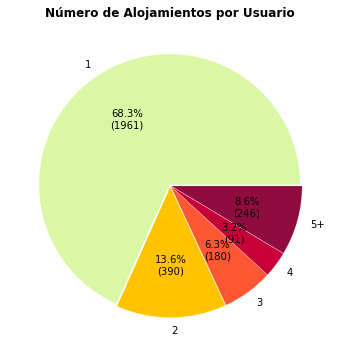
\includegraphics[width=0.45\textwidth]{capturas/12.png}
    \captionof{figure}{Número de alojamientos por usuario.}
\end{center}
\begin{center}
    \centering
    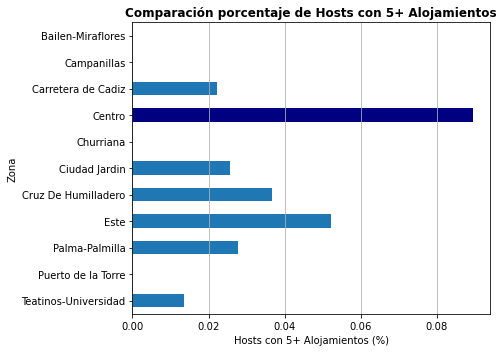
\includegraphics[width=0.7\textwidth]{capturas/13.png}
    \captionof{figure}{Comparación porcentaje de Hosts con +5 alojamientos.}
\end{center}
Vemos que el distrito \textit{Centro} un 10\% de los propietarios tiene más de 5 alojamientos publicados en Airbnb. Es interesante notar que un porcentaje significativo de propietarios tiene múltiples propiedades, lo que puede sugerir una tendencia hacia el negocio de alquileres a corto plazo en la ciudad. Este dato puede ser relevante para el mercado inmobiliario y la industria turística, ya que muestra el nivel de participación de ciertos propietarios en el mercado de alquileres vacacionales.

\subsection{Consulta de cuántos hosts se unen cada año}
La consulta tiene como objetivo mostrar cuántos hosts (propietarios) se unen cada año en Airbnb en la ciudad de Málaga. Estos datos son útiles para comprender la evolución del mercado de alquileres vacacionales en la ciudad y pueden ser útiles para las autoridades locales y profesionales del sector turístico para tomar decisiones y adaptar sus estrategias en función de las tendencias y cambios en la plataforma.
\begin{verbatim}
SELECT EXTRACT(YEAR FROM host_since) AS joined_year, 
    COUNT(DISTINCT host_id) AS new_hosts
FROM listings
GROUP BY joined_year
ORDER BY joined_year;
\end{verbatim}
\begin{table}[h]
\centering
\begin{tabular}{|l|r|}
\hline
\textbf{Año de Unión} & \textbf{Nuevos Hosts} \\
\hline
2009 & 1 \\ \hline
2010 & 1 \\ \hline
2011 & 26 \\ \hline
2012 & 88 \\ \hline
2013 & 140 \\ \hline
2014 & 246 \\ \hline
2015 & 357 \\ \hline
2016 & 422 \\ \hline
2017 & 360 \\ \hline
2018 & 283 \\ \hline
2019 & 280 \\ \hline
2020 & 132 \\ \hline
2021 & 184 \\ \hline
2022 & 282 \\ \hline
2023 & 70 \\ \hline
\end{tabular}
\caption{Número de nuevos hosts que se unieron cada año en Airbnb en Málaga.}
\end{table}

El resultado de la consulta nos muestra que ha habido un crecimiento notable a lo largo de los años fruto de la incipiente popularidad de esta plataforma. Sugiere además un crecimiento continuo de la oferta de alojamientos en la plataforma en la ciudad.

\subsection{Consulta de porcentaje y nº camas por alojamiento}
Esta consulta muestra el porcentaje de alojamientos en Málaga según el número de camas que ofrecen, así como la cantidad absoluta de alojamientos en cada categoría. El objetivo es comprender la distribución de camas en la oferta de alojamientos en la ciudad. Los resultados obtenidos son los siguientes:
\begin{verbatim}
SELECT beds, COUNT(*) AS count, 
    ROUND(COUNT(*) * 100.0 / (SELECT COUNT(*) FROM listings), 2) AS percentage
FROM listings
GROUP BY beds
ORDER BY percentage DESC;
\end{verbatim}
\begin{table}[h]
\centering
\begin{tabular}{|l|r|r|}
\hline
\textbf{Número de Camas} & \textbf{Cantidad} & \textbf{Porcentaje (\%)} \\ \hline
1 & 2308 & 30.63 \\ \hline
2 & 2248 & 29.84 \\ \hline
3 & 1370 & 18.18 \\ \hline
4 & 833 & 11.06 \\ \hline
5 & 326 & 4.33 \\ \hline
6 & 167 & 2.22 \\ \hline
7 & 79 & 1.05 \\ \hline
8 & 44 & 0.58 \\ \hline
9 & 26 & 0.35 \\ \hline
10 & 31 & 0.41 \\ \hline
... & ... & ... \\ \hline
\end{tabular}
\caption{Porcentaje y número de camas por alojamiento en Málaga.}
\end{table}
\newpage
La tabla muestra que la mayoría de los alojamientos en Málaga ofrecen 1 o 2 camas, representando aproximadamente el 60.47\% del total. Por otro lado, los alojamientos con más de 4 camas son menos comunes, y los que ofrecen 6 camas o más representan menos del 6\% del total. Estos datos son útiles para entender la capacidad y distribución de alojamientos disponibles para los viajeros en Málaga.

\subsection{Consulta de porcentaje de precio}
Esta consulta proporciona información sobre la distribución de los precios de alojamientos en Málaga y su frecuencia relativa.
Los resultados obtenidos son los siguientes:

\begin{table}[h]
\centering
\begin{tabular}{|l|r|r|}
\hline
\textbf{Precio} & \textbf{Cantidad} & \textbf{Porcentaje (\%)} \\ \hline
56.00 \texteuro & 148 & 1.96 \\ \hline
150.00 \texteuro & 124 & 1.65 \\ \hline
100.00 \texteuro & 123 & 1.63 \\ \hline
120.00 \texteuro & 110 & 1.46 \\ \hline
90.00 \texteuro & 91 & 1.21 \\ \hline
60.00 \texteuro & 78 & 1.04 \\ \hline
70.00 \texteuro & 78 & 1.04 \\ \hline
80.00 \texteuro & 76 & 1.01 \\ \hline
200.00 \texteuro & 72 & 0.96 \\ \hline
65.00 \texteuro & 66 & 0.88 \\ \hline
... & ... & ... \\ \hline
\end{tabular}
\caption{Porcentaje de precio de alojamientos en Málaga.}
\end{table}

La tabla muestra la distribución de los precios de alojamientos en Málaga y su frecuencia relativa en la base de datos. El precio modal es 56.00 € con una frecuencia relativa del 1.96\%. Es interesante observar cómo los precios se distribuyen a lo largo de diferentes rangos y cómo la mayoría de los precios tienen una frecuencia baja, lo que indica una diversidad de opciones de alojamiento para los visitantes.\\\\
Además, se presentan dos visualizaciones gráficas que profundizan en la distribución de los precios de los alojamientos:
\newpage
Esta figura muestra la distribución de precios de alojamientos en Málaga. Es evidente que la concentración de datos en el rango más bajo y la dispersión en los rangos superiores hacen que la gráfica sea difícil de interpretar. Algunos valores atípicos extremos pueden estar afectando la visualización.
\begin{center}
    \centering
    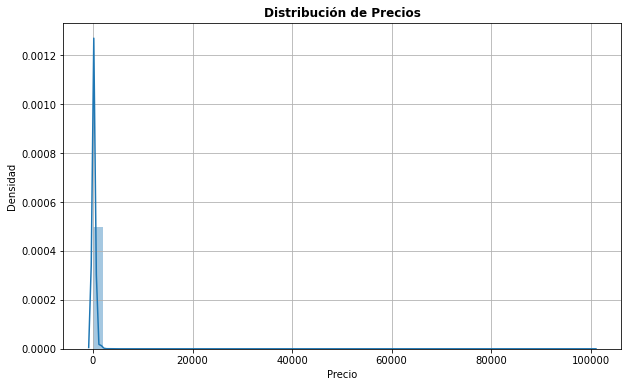
\includegraphics[width=1\textwidth]{capturas/15.png}
    \captionof{figure}{Distribución de Precios.}
\end{center}
Para abordar la concentración en la parte inferior de la gráfica, se ha aplicado una transformación logarítmica a los precios. Esto ayuda a suavizar la visualización y hacer que los datos sean más comprensibles. La gráfica presenta una distribución más uniforme de los precios en comparación con la gráfica anterior.
\begin{center}
    \centering
    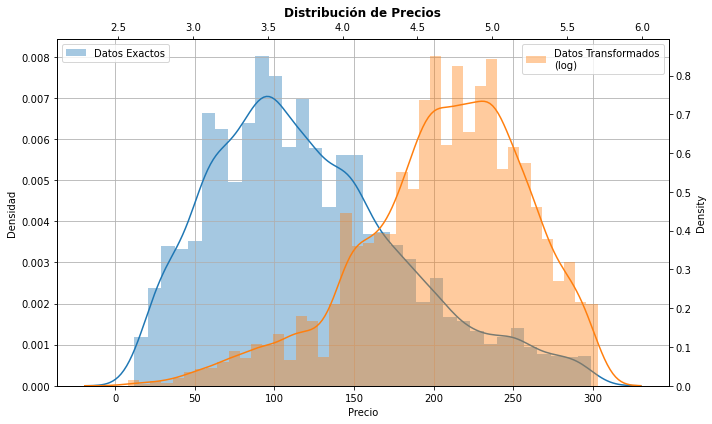
\includegraphics[width=1\textwidth]{capturas/16.png}
    \captionof{figure}{Distribución de Precios (log).}
\end{center}
\subsection{Porcentaje de mínimo numero de noches}
La siguiente consulta muestra el porcentaje de alojamientos en Málaga según el número mínimo de noches requerido para reservar:
Los resultados obtenidos son los siguientes:

\begin{table}[h]
\centering
\begin{tabular}{|l|r|r|}
\hline
\textbf{Mínimo de Noches} & \textbf{Cantidad} & \textbf{Porcentaje (\%)} \\ \hline
3 & 6350 & 82,29 \\ \hline
4 & 457 & 6.07 \\ \hline
5 & 271 & 3.60 \\ \hline
7 & 153 & 2.03 \\ \hline
30 & 70 & 0.93 \\ \hline
6 & 70 & 0.93 \\ \hline
60 & 51 & 0.68 \\ \hline
10 & 19 & 0.25 \\ \hline
28 & 14 & 0.19 \\ \hline
15 & 13 & 0.17 \\ \hline
32 & 9 & 0.12 \\ \hline
61 & 8 & 0.11 \\ \hline
... & ... & ... \\ \hline
\end{tabular}
\caption{Porcentaje de mínimo número de noches en alojamientos de Málaga.}
\end{table}

Podemos observar que la mayoría de los alojamientos en Málaga tienen un mínimo de 3 noches requeridas para reservar, representando el 82,29\%. Los mínimos de 4, 5 y 6 noches también son comunes, mientras que los mínimos más largos (30, 60, etc.) tienen un porcentaje mucho menor en la oferta de alojamientos.

\subsection{Porcentaje de puntuaciones}
La siguiente consulta muestra el porcentaje de puntuaciones en los alojamientos de Málaga:
\begin{verbatim}
SELECT review_scores_rating, COUNT(*) AS count, 
    ROUND(COUNT(*) * 100.0 / (SELECT COUNT(*) FROM listings), 2) 
        AS percentage
FROM listings WHERE review_scores_rating IS NOT NULL
GROUP BY review_scores_rating
ORDER BY percentage DESC;
\end{verbatim}
\begin{table}[h]
\centering
\begin{tabular}{|l|r|r|}
\hline
\textbf{Puntuación} & \textbf{Cantidad} & \textbf{Porcentaje (\%)} \\ \hline
5.00 & 1061 & 14.08 \\ \hline
4.50 & 248 & 3.29 \\ \hline
4.00 & 239 & 3.17 \\ \hline
4.67 & 208 & 2.76 \\ \hline
4.75 & 148 & 1.96 \\ \hline
4.83 & 134 & 1.78 \\ \hline
4.80 & 118 & 1.57 \\ \hline
4.88 & 108 & 1.43 \\ \hline
... & ... & ... \\ \hline
\end{tabular}
\caption{Porcentaje de puntuaciones en alojamientos de Málaga.}
\end{table}

Encontramos que la mayoría de los alojamientos en Málaga tienen una puntuación de 5.00 (la calificación más alta posible), representando el 14.08\% del total de alojamientos. También es notable la presencia de puntuaciones en torno a 4.0 y 4.5, aunque con porcentajes menores. La distribución de las puntuaciones muestra una tendencia hacia calificaciones altas, lo que sugiere que la mayoría de los alojamientos en Málaga son bien valorados por los huéspedes.

\subsection{Consulta de media de precios de alojamiento en función de su valoracion}
La siguiente consulta muestra la media de precios de los alojamientos en Málaga según su valoración. \\
A continuación se muestra el código de la vista y un fragmento de los resultados:
\begin{verbatim}
SELECT rating_range, 
    ROUND(AVG(CAST(REGEXP_REPLACE(price, '[^\d.]', '', 'g')
        AS NUMERIC)), 2) AS average_price
FROM ( SELECT 
    CASE
      WHEN review_scores_rating BETWEEN 0 AND 1 THEN '0-1'
      WHEN review_scores_rating > 1 AND review_scores_rating <= 2 THEN '1-2'
      WHEN review_scores_rating > 2 AND review_scores_rating <= 3 THEN '2-3'
      WHEN review_scores_rating > 3 AND review_scores_rating <= 4 THEN '3-4'
      WHEN review_scores_rating > 4 AND review_scores_rating <= 5 THEN '4-5' END 
    AS rating_range, 
    price
    FROM listings
    WHERE review_scores_rating IS NOT NULL
    ) AS subquery
GROUP BY rating_range
ORDER BY rating_range;
\end{verbatim}
Los resultados obtenidos son los siguientes:

\begin{table}[h]
\centering
\begin{tabular}{|l|r|}
\hline
\textbf{Valoración} & \textbf{Precio Medio} \\ \hline
0-1 & 154.77 \texteuro \\ \hline
1-2 & 136.25 \texteuro\\ \hline
2-3 & 609.79 \texteuro\\ \hline
3-4 & 300.56 \texteuro\\ \hline
4-5 & 187.05 \texteuro\\ \hline
\end{tabular}
\caption{Media de precios de alojamiento en función de su valoración en Málaga.}
\end{table}

Se observa que los alojamientos con una valoración de 2 a 3 tienen un precio medio excepcionalmente alto en comparación con otras categorías de valoración, mientras que aquellos con una valoración de 1 a 2 y 4 a 5 tienden a tener precios medios más bajos. \\Estos resultados sugieren que los alojamientos mejor valorados y peor valorados en Málaga pueden ofrecer una mejor relación calidad-precio en términos de precios promedio.
\ \\\\
A continuación, exploramos una gráfica que arroja luz sobre la relación entre el número de reseñas y los precios de los alojamientos en Málaga. Esta visualización proporciona información valiosa sobre cómo la popularidad y la valoración de un alojamiento pueden influir en su precio promedio. Muestra cómo esta relación podría tener implicaciones para los anfitriones y los huéspedes.
\begin{center}
    \centering
    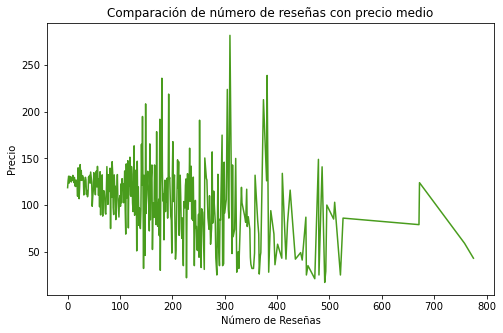
\includegraphics[width=1\textwidth]{capturas/17.png}
    \captionof{figure}{Comparación de número de reseñas y precios.}
\end{center}
La fluctuación de precios en función del número de reseñas sugiere que existe una relación compleja entre la popularidad de un alojamiento y su precio promedio. Se observa que, en general, alojamientos con alrededor de 100 reseñas tienden a tener precios medios que oscilan entre 80 y 130 euros. A medida que el número de reseñas aumenta, los precios también fluctúan considerablemente. Por ejemplo, alojamientos con alrededor de 300 reseñas varían en precio desde 80 euros hasta más de 200 euros. Sin embargo, en el rango de 600-700 reseñas, la variabilidad es menor, con precios estabilizándose en torno a 100 euros o 130 euros. Esto puede deberse a que haya una menor muestra de alojamientos con tantas reseñas.
\newpage